\chapter{Statistical Analysis}
To estimate the sensibility of the $tH$ signal, we define an Asimov dataset, made by replacing the ensemble of simulated backgrounds and signal by a single one. The statistical uncertainty of the Asimov data is calculated as $\sqrt{n}$, with $n$ the number of events. The uncertainty of the signal strength is estimated by applying a  fit to the Asimov dataset, where the model
is constructed from the sum of the individual backgrounds and signal. The fit is implemented using a Poisson likelihood and gaussian constraints for the systematical uncertainties in the model.


\section{Likelihood and fit procedure}
The likelihood function is the product of Poisson probabilities for all bins of the BDT distribution. The likelihood function has the form
\begin{align}
L(\mu,\alpha)=\prod_{j=1}^{N}\frac{(\mu s_j +b_j)^{n_j}}{n_j !}e^{-(\mu s_j+b_j)} \prod_{k=1}^M e^{\frac{-\alpha^2_k}{2}}
\end{align}
where $N$ is the total number of bins, n is the number of events in a bin $j$,  $s_j$ is the number of signal events, $\mu$ is the parameter of signal strength and  $b_j$ is the number of background events.
$b_j$ is the sum of different background processes $k$
\begin{align}
b_j=\sum_k b_j^k(1+\sigma_k \alpha)
\end{align}
$\alpha$ is the parameter that modifies the expected background prediction and $\sigma_k$ is the systematic uncertainty of the associated background. \\

The fit is applied by minimizing the $-\log{L}$ (NLL) with respect to the parameter $\mu$ and $\alpha_k$. The minimization is performed by using the package ROOFIT \cite{roofit}.
%log es usado para evitar valores extremadamente pequenos debido a los productos de los exponenciales
%negativo es para hacer una minimizacion, positivo es maximizacion
\pagebreak

\begin{table}[ht!]
	\centering
	\caption{Postfit for each yield.Prefit uncertainty is statistical only. Postfit uncertainty is statistical + systematic.}
\begin{tabular}{ccc}
	\hline
	Process  & SM    & $k_t=-1$ \\
	\hline
$t\bar{t}W$  &  68$\pm$8.9& 68 $\pm$8.9 \\
	$t\bar{t}Z$  & 25.9$\pm$3.8&25.9$\pm$3.8\\
$WZ$ &  15.1$\pm$7.4& 15.1$\pm$7.4\\
Rares &  20.8$\pm$4.8& 20.8$\pm$4.8 \\
	Fakes  &  80.9$\pm$9.0&  80.9$\pm$8.9 \\
	$t\bar{t}H$  &   24.2$\pm$2.0 &  24.2$\pm$2.0 \\
\hline
$tH$&  2.14$\pm$16.56 &26.22$\pm$13.11 
\end{tabular}
\label{table1}
\end{table}

In the figure \ref{simple} and table \ref{table1} , shows the results of the model fitting using the Asimov data for both models. As mentioned before, the  $k_t=-1$, the number of events for the $tH$ signal is more than ten times, compared to SM. This causes that the fit model have access to more data, and so improve the fit a bit. Due to low $tH$ number of events, the uncertainty after the fit is big, compared to the $k_t=-1$ model, where the uncertainty is around 50$\%$. Because of the model, the values of the backgrounds don't change.
\begin{figure}[!htbp]
	\centering
	\begin{minipage}[b]{0.48\textwidth}
		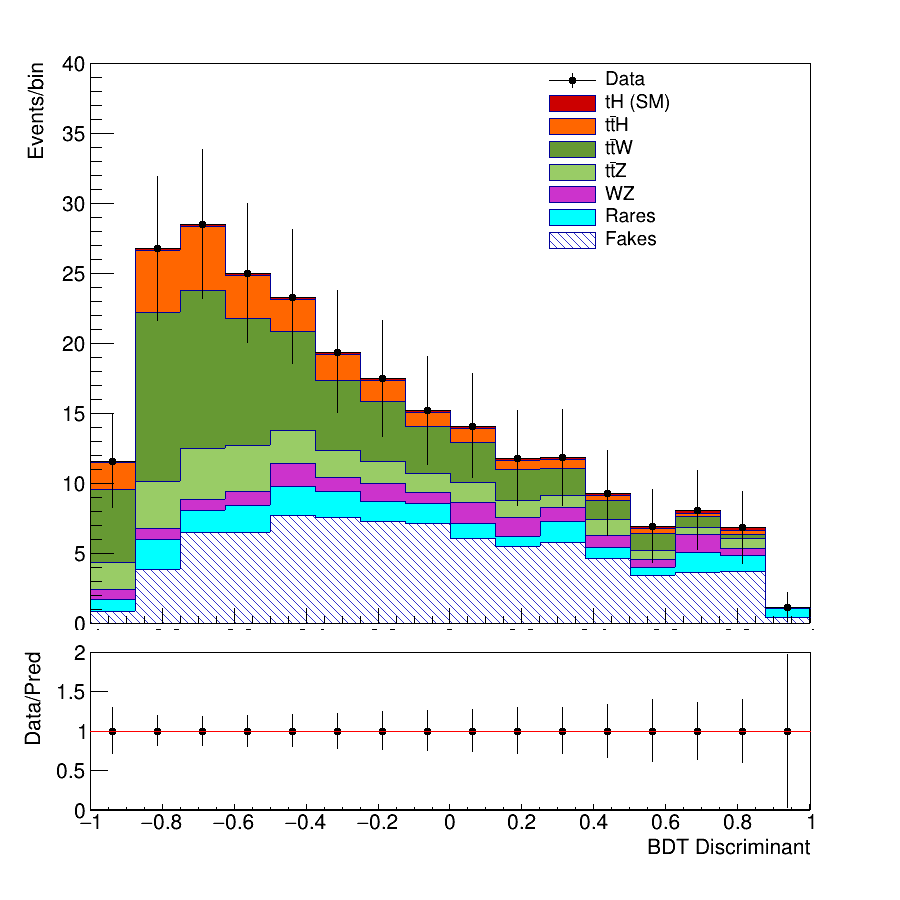
\includegraphics[width=\textwidth]{Chapter4/simple.png}
	\end{minipage}
	\hfill
	\begin{minipage}[b]{0.48\textwidth}
		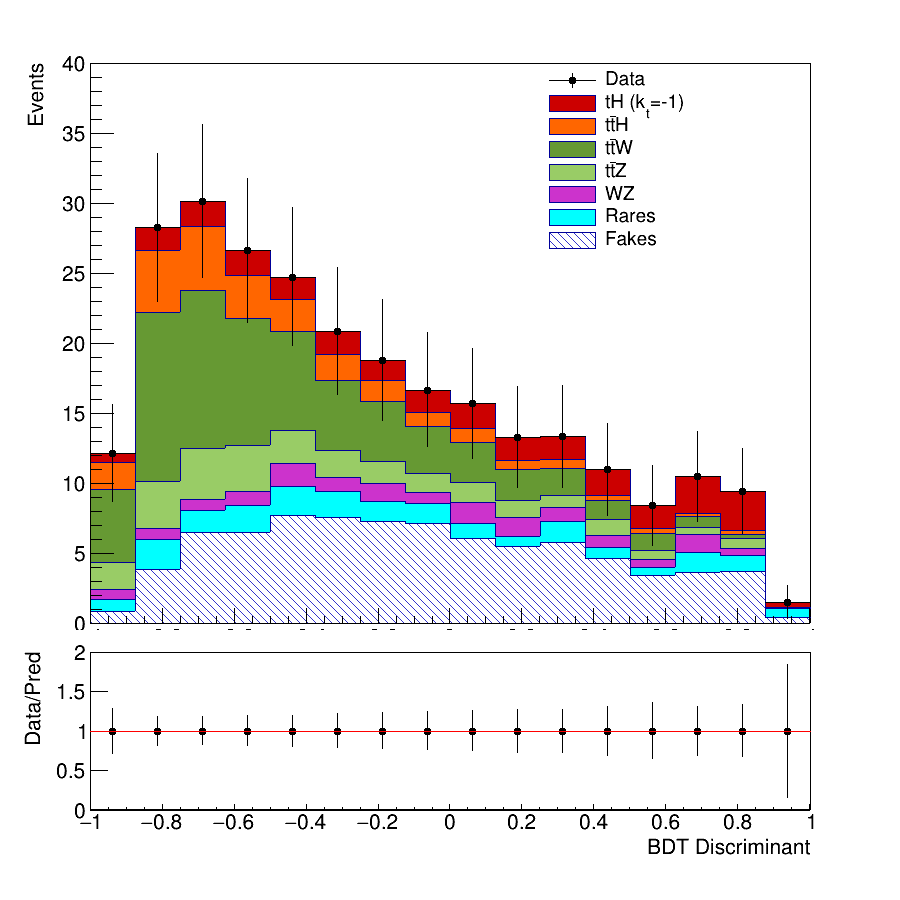
\includegraphics[width=\textwidth]{Chapter4/simple-kt-1.png}
	\end{minipage}
	\caption{Post fit signal and background yields for tH process for SM (Left) and $k_t=-1$ (Right).
		In the box below each distribution, the ratio of the observed and predicted event yields is shown}
\label{simple}
\end{figure}
In the table \ref{parameters}, shows the $\mu$ and $\alpha$ parameters. For the pre-fit, values of $\alpha$ are set to zero and $\mu$ is set to 1.After the fit,  $\alpha$ parameters set to zero indicates that in the fit, the values of the backgrounds didn't changed for the SM and the $\mu$ parameter set to 1 indicates that the signal strength also didn't changed, but its uncertainty is also big.
However, in the model $k_t=-1$, the $\alpha$ parameters shows a slightly change, that indicates changes in the backgrounds, but with a great uncertainty. For the $\mu$, it shows the same size, but the uncertainty is estimated to be 50$\%$, corresponding to the results obtained for the events yields.
\begin{table}[ht]
	\centering
	\caption{$\alpha$ and $\mu$ values for 35.9 fb$^{-1}$}
	\begin{tabular}{ccc}
		\hline
		Parameter  & SM &kt\\
		$\mu$   & 1.00 $\pm$  7.74& 1.0 $\pm$  0.5\\
		$alpha_ttw$&  0.00 $\pm$  0.89&  6.32$\times 10^{-09}$ $\pm$  089\\
		$alpha_ttz$ &  0.00 $\pm$  0.98& 1.90$\times 10^{-09}$ $\pm$  0.98\\
		$alpha_wz$   & 0.00 $\pm$  0.97& -5.33$\times 10^{-09}$9 $\pm$  0.97\\
		$alpha_tz$   &0.00 $\pm$  0.95&-7.83$\times 10^{-09}$ $\pm$  0.98 \\
		$alpha_fakes$ &   0.00 $\pm$  0.96&  3.47 $\times 10^{-09}$ $\pm$  0.95\\
		$alpha_tth$ &0.00 $\pm$  0.98& 2.61$\times 10^{-09}$ $\pm$ 0.98\\
	\end{tabular}
\label{parameters}
\end{table}

For the analysis of the likelihood function,  we take likelihood ratio
\begin{align}
	\lambda(\mu,\theta(\mu))=\frac{L(\mu,\hat{\hat{\theta}}(\mu))}{L(\hat{\mu},\hat{\theta}(\mu))}
\end{align}
Where $\hat{\hat{\theta}}(\mu) $ in the numerator denotes the value of $\theta(\mu)$ that maximizes L for the specified $\mu$, that is , the conditional maximum-likelihood (ML) estimator of $\hat{\theta}(\mu)$ 
The denominator represents the  maximized  likelihood function, where $\hat{\mu}$ and $\hat{\theta}$ are
their ML estimators.
The presence of the nuisance parameters broadens the profile likelihood as a
function of $\mu$ relative to what one would have if their values were fixed. This reflects the loss
of information about $\mu$ due to the systematic uncertainties

\section{Limit calculation}
Due to the large background, the signal strength for the Asimov data with 35.9 $fb^{-1}$ is consistency with zero.
Therefore, we estimate an upper limit on the signal strenght at 95 $\%$ level of confidence.








For purposes of establishing an upper limit on the strength parameter $\mu$ , we consider two
closely related test statistics. First, we may define
\begin{align}
q_{\mu}=  \Big\{    \begin{array}{ll}
-2\ln\lambda(\mu) \qquad \hat{\mu} \leq \mu	\\
0  \qquad \qquad \qquad \hat{\mu}< 0
\end{array}
\end{align}
The reason for setting $q_\mu = 0$
for $\hat{\mu}>\mu $ is that when setting an upper limit, one would not regard data with $\hat{\mu}>\mu $ as
representing less compatibility with $\mu$ than the data obtained, and therefore this is not taken
as part of the rejection region of the test. From the definition of the test statistic one sees that
higher values of $q_\mu$ represent greater incompatibility between the data and the hypothesized
value of $\mu$.



\begin{table}[ht!]
	\caption{Estimation of $\mu$ and upper limits  for extrapolations}
	\begin{tabular}{|c|c|c|c|c|}
		\hline
		Luminosity (fb$^{-1}$)	&$\mu$ &$\mu$ for $k_t=-1$ &$\mu$ upper limit &$\mu$ upper limit for $k_t=-1$ \\
		\hline
		35.9 & 1.00 $\pm$  8.32 & 1.00 $\pm$  0.249&	22.328 & 2.777   \\
		\hline
		150& 1.00 $\pm$  6.44 & 1.00 $\pm$  0.544  &12.619 &0.915 \\
		\hline
		300&1.00 $\pm$  4.83 &1.00 $\pm$  0.407 & 9.427&0.649 \\
		\hline
		3000&1.00 $\pm$  1.54 & 1.00 $\pm$  0.151&	 3.442 & 0.25
		\\
		\hline
	\end{tabular}
\end{table}


